\documentclass{beamer}
\usepackage[T2A]{fontenc}
\usepackage[utf8]{inputenc}
\usepackage[english,russian]{babel}
\usepackage{amssymb,amsfonts,amsmath,mathtext}
\usepackage{cite,enumerate,float,indentfirst}

\usetheme{Warsaw}

\title{Отчет по 2-му заданию}
\author{Масло Михаил, Лазарев Владимир, Подкина Александра}
\institute{МГУ имени М. В. Ломоносова}
\date{Москва, 2017}

\begin{document}

%%титульная страница
\maketitle

\begin{frame}
\frametitle{Введение}
\begin{flushleft}
\small{В отличие от традиционной проверки гипотез, предназначенной для проверки априорных предположений, касающихся связей между переменными (например, "Имеется положительная корреляция между возрастом человека и его/ее нежеланием рисковать"), разведывательный анализ данных (РАД) применяется для нахождения связей между переменными в ситуациях, когда отсутствуют (или недостаточны) априорные представления о природе этих связей. Как правило, при разведочном анализе учитывается и сравнивается большое число переменных, а для поиска закономерностей используются самые разные методы.}
\end{flushleft}
\begin{center}
\begin{block}{Типичные техники, используемые в РАД}
\begin{itemize}
\item Диаграмма размаха(Boxplot)
\item Гистограмма
\item Многовариантный график
\item Диаграмма "стебель-листья" и др.
\end{itemize}
\end{block}
\end{center}
\end{frame}

\begin{frame}
\begin{flushleft}
\frametitle{Анализ}
\framesubtitle{Чтение исходных данных}
\small{В качестве исходных данных мы имеем информацию о производстве оружия и количестве единиц сломанного оружия за каждый месяц каждым из кузнецов. Верхние строки этой таблицы выглядят так:}
\end{flushleft}
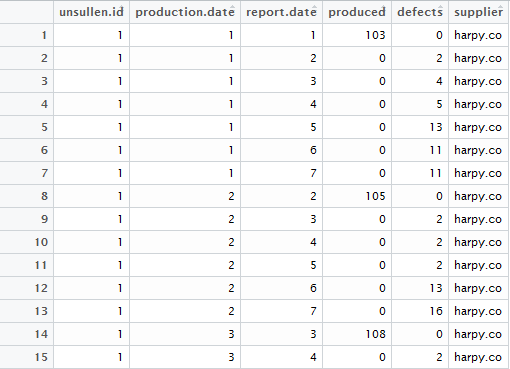
\includegraphics[width=1\linewidth]{images/image1.png}
\end{frame}

\begin{frame}
\frametitle{Анализ}
\framesubtitle{Процент дефекта}
\small{В качестве показателя, на основании которого будет приниматься итоговое решение о выборе компании, возьмем процент дефектных орудий для каждой произведенной партии. Покажем как выглядят первые строки получившихся таблиц для двух компаний.}
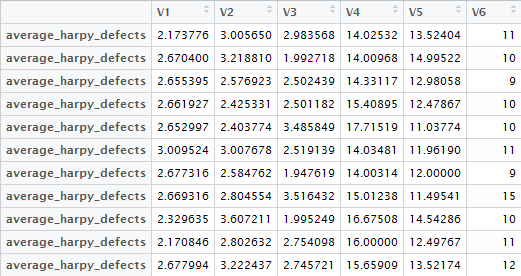
\includegraphics[width=1\linewidth]{images/image2.png}
\end{frame}

\begin{frame}
\frametitle{Анализ}
\framesubtitle{Таблица с процентами дефектных орудий}
\small{Каждый столбец отвечает за конкретный месяц после производства. Каждая
строка соответствует одному кузнецу.}
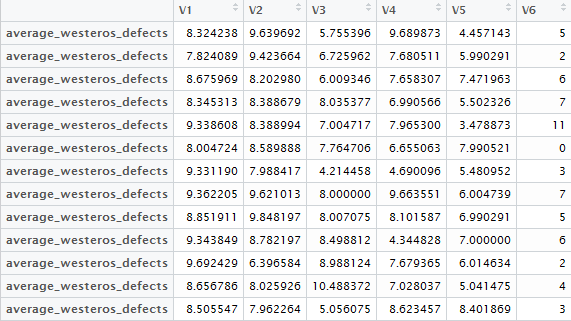
\includegraphics[width=1\linewidth]{images/image3.png}
\end{frame}

\begin{frame}
\begin{flushleft}
\frametitle{Анализ}
\framesubtitle{Диаграмма размаха}
\small{Наш анализ будет строиться на основе диаграммы размаха(boxplot). Дадим формализацию этого понятия.}
\begin{block}{Диаграмма размаха}
\scriptsize{Диаграмма размаха - график, использующийся в описательной статистике, компактно изображающий одномерное распределение вероятностей. Такой вид диаграммы в удобной форме показывает медиану (или, если нужно, среднее), нижний и верхний квартили, минимальное и максимальное значение выборки и выбросы. Несколько таких диаграмм можно нарисовать бок о бок, чтобы визуально сравнивать одно распределение с другим; их можно располагать как горизонтально, так и вертикально. Расстояния между различными частями ящика позволяют определить степень разброса (дисперсии) и асимметрии данных и выявить выбросы.}
\end{block}
\end{flushleft}
\end{frame}

\begin{frame}
\begin{flushleft}
\frametitle{Анализ}
\framesubtitle{Диаграмма размаха Harpy}
\small{Изобразим наши получившиеся данные в виде boxplot графиков, чтобы более
наглядно увидеть различия в компаниях. Сначала изобразим boxplot для Harpy и дадим некоторые комментарии увиденному.}
\end{flushleft}
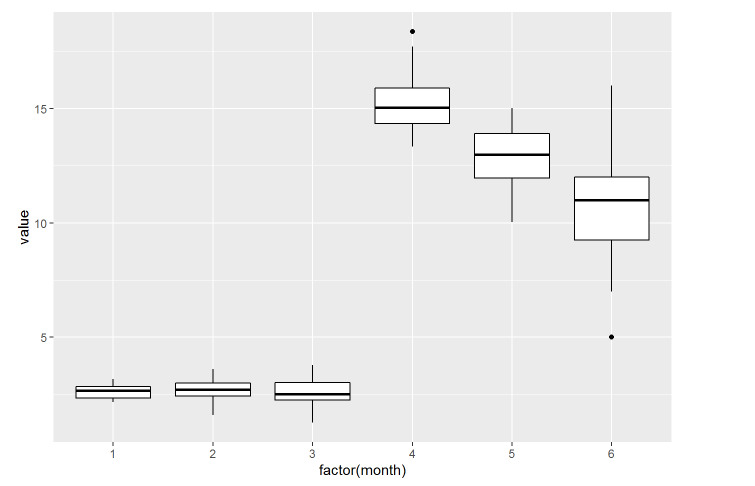
\includegraphics[width=1\linewidth]{images/image4.png}
\end{frame}

\begin{frame}
\begin{flushleft}
\frametitle{Анализ}
\framesubtitle{Анализ Harpy}
\small{Первые 3 месяца показывают относительно идентичную динамику, т.е. дефекты более менее одинаковые(различие наблюдаются в разнице между high и low значениями, high - low имеет линейную динамику роста). Но на 4-й месяц происходит резкое изменение, что говорит о том, что в 4-м месяце достигается глобальный максимум поломки орудий. Далее, наблюдается линейное убывание дефектов по среднему значению.}
\end{flushleft}
\end{frame}

\begin{frame}
\begin{flushleft}
\frametitle{Анализ}
\framesubtitle{Диаграмма размаха Westeros}
\end{flushleft}
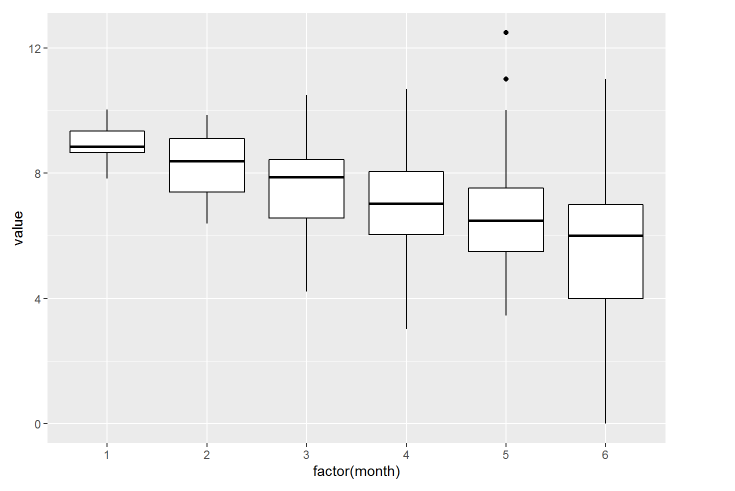
\includegraphics[width=1\linewidth]{images/image5.png}
\end{frame}

\begin{frame}
\begin{flushleft}
\frametitle{Анализ}
\framesubtitle{Анализ Westeros}
\small{Здесь мы видим следующее. Дефекты напоминают линейную функцию, убывающую с ростом месяца. В данном случае и среднее значение, и дисперсия показывает линейную динамику, что является очень привлекательным фактом для прогноза процентов дефекта на 
будущее. Простая линейная регрессия вполне может дать валидные результаты, 
чего нельзя сказать с уверенностью про компанию Harpy.}
\end{flushleft}
\end{frame}

\begin{frame}
\begin{flushleft}
\frametitle{Анализ}
\framesubtitle{Итоги}
\small{Обе компании имеют как положительные, так и отрицательные стороны. Компания Harpy показывает гораздо более низкую дисперсию по проценту дефекта в первые 3 месяца по сравнению с компанией Westeros. Это позволяет нам лучше прогнозировать поломки орудий на первые 3 месяца после производства партии. Но наш горизонт планирования составляет 11 месяцев, т.е. значительно больше 3 месяцев. На этом временном промежутке преимущество по дисперсии стирается, так как на 4-6 месяцы, судя по имеющимся результатам, дисперсия возрастает и становится вполне сравнимой с компанией Westeros. Компания Westeros в свою очередь имеет линейную динамику как по среднему значению, так и по дисперсии, что свидетельствует о большей вероятности сохранения “тренда”. Это хорошее подспорье для валидности прогноза на наш горизонт планирования. В качестве минуса Westeros можно отметить большое расстояние между high и low значениями в каждый месяц после производства. Несмотря на это привлекательность компании Westeros выше Harpy, поэтому контракт выгоднее заключить с Westeros.}
\end{flushleft}
\end{frame}

\end{document} 